% Options for packages loaded elsewhere
\PassOptionsToPackage{unicode}{hyperref}
\PassOptionsToPackage{hyphens}{url}
\PassOptionsToPackage{dvipsnames,svgnames,x11names}{xcolor}
%
\documentclass[
]{interact}

\usepackage{amsmath,amssymb}
\usepackage{iftex}
\ifPDFTeX
  \usepackage[T1]{fontenc}
  \usepackage[utf8]{inputenc}
  \usepackage{textcomp} % provide euro and other symbols
\else % if luatex or xetex
  \usepackage{unicode-math}
  \defaultfontfeatures{Scale=MatchLowercase}
  \defaultfontfeatures[\rmfamily]{Ligatures=TeX,Scale=1}
\fi
\usepackage{lmodern}
\ifPDFTeX\else  
    % xetex/luatex font selection
\fi
% Use upquote if available, for straight quotes in verbatim environments
\IfFileExists{upquote.sty}{\usepackage{upquote}}{}
\IfFileExists{microtype.sty}{% use microtype if available
  \usepackage[]{microtype}
  \UseMicrotypeSet[protrusion]{basicmath} % disable protrusion for tt fonts
}{}
\makeatletter
\@ifundefined{KOMAClassName}{% if non-KOMA class
  \IfFileExists{parskip.sty}{%
    \usepackage{parskip}
  }{% else
    \setlength{\parindent}{0pt}
    \setlength{\parskip}{6pt plus 2pt minus 1pt}}
}{% if KOMA class
  \KOMAoptions{parskip=half}}
\makeatother
\usepackage{xcolor}
\setlength{\emergencystretch}{3em} % prevent overfull lines
\setcounter{secnumdepth}{5}
% Make \paragraph and \subparagraph free-standing
\makeatletter
\ifx\paragraph\undefined\else
  \let\oldparagraph\paragraph
  \renewcommand{\paragraph}{
    \@ifstar
      \xxxParagraphStar
      \xxxParagraphNoStar
  }
  \newcommand{\xxxParagraphStar}[1]{\oldparagraph*{#1}\mbox{}}
  \newcommand{\xxxParagraphNoStar}[1]{\oldparagraph{#1}\mbox{}}
\fi
\ifx\subparagraph\undefined\else
  \let\oldsubparagraph\subparagraph
  \renewcommand{\subparagraph}{
    \@ifstar
      \xxxSubParagraphStar
      \xxxSubParagraphNoStar
  }
  \newcommand{\xxxSubParagraphStar}[1]{\oldsubparagraph*{#1}\mbox{}}
  \newcommand{\xxxSubParagraphNoStar}[1]{\oldsubparagraph{#1}\mbox{}}
\fi
\makeatother

\usepackage{color}
\usepackage{fancyvrb}
\newcommand{\VerbBar}{|}
\newcommand{\VERB}{\Verb[commandchars=\\\{\}]}
\DefineVerbatimEnvironment{Highlighting}{Verbatim}{commandchars=\\\{\}}
% Add ',fontsize=\small' for more characters per line
\usepackage{framed}
\definecolor{shadecolor}{RGB}{241,243,245}
\newenvironment{Shaded}{\begin{snugshade}}{\end{snugshade}}
\newcommand{\AlertTok}[1]{\textcolor[rgb]{0.68,0.00,0.00}{#1}}
\newcommand{\AnnotationTok}[1]{\textcolor[rgb]{0.37,0.37,0.37}{#1}}
\newcommand{\AttributeTok}[1]{\textcolor[rgb]{0.40,0.45,0.13}{#1}}
\newcommand{\BaseNTok}[1]{\textcolor[rgb]{0.68,0.00,0.00}{#1}}
\newcommand{\BuiltInTok}[1]{\textcolor[rgb]{0.00,0.23,0.31}{#1}}
\newcommand{\CharTok}[1]{\textcolor[rgb]{0.13,0.47,0.30}{#1}}
\newcommand{\CommentTok}[1]{\textcolor[rgb]{0.37,0.37,0.37}{#1}}
\newcommand{\CommentVarTok}[1]{\textcolor[rgb]{0.37,0.37,0.37}{\textit{#1}}}
\newcommand{\ConstantTok}[1]{\textcolor[rgb]{0.56,0.35,0.01}{#1}}
\newcommand{\ControlFlowTok}[1]{\textcolor[rgb]{0.00,0.23,0.31}{\textbf{#1}}}
\newcommand{\DataTypeTok}[1]{\textcolor[rgb]{0.68,0.00,0.00}{#1}}
\newcommand{\DecValTok}[1]{\textcolor[rgb]{0.68,0.00,0.00}{#1}}
\newcommand{\DocumentationTok}[1]{\textcolor[rgb]{0.37,0.37,0.37}{\textit{#1}}}
\newcommand{\ErrorTok}[1]{\textcolor[rgb]{0.68,0.00,0.00}{#1}}
\newcommand{\ExtensionTok}[1]{\textcolor[rgb]{0.00,0.23,0.31}{#1}}
\newcommand{\FloatTok}[1]{\textcolor[rgb]{0.68,0.00,0.00}{#1}}
\newcommand{\FunctionTok}[1]{\textcolor[rgb]{0.28,0.35,0.67}{#1}}
\newcommand{\ImportTok}[1]{\textcolor[rgb]{0.00,0.46,0.62}{#1}}
\newcommand{\InformationTok}[1]{\textcolor[rgb]{0.37,0.37,0.37}{#1}}
\newcommand{\KeywordTok}[1]{\textcolor[rgb]{0.00,0.23,0.31}{\textbf{#1}}}
\newcommand{\NormalTok}[1]{\textcolor[rgb]{0.00,0.23,0.31}{#1}}
\newcommand{\OperatorTok}[1]{\textcolor[rgb]{0.37,0.37,0.37}{#1}}
\newcommand{\OtherTok}[1]{\textcolor[rgb]{0.00,0.23,0.31}{#1}}
\newcommand{\PreprocessorTok}[1]{\textcolor[rgb]{0.68,0.00,0.00}{#1}}
\newcommand{\RegionMarkerTok}[1]{\textcolor[rgb]{0.00,0.23,0.31}{#1}}
\newcommand{\SpecialCharTok}[1]{\textcolor[rgb]{0.37,0.37,0.37}{#1}}
\newcommand{\SpecialStringTok}[1]{\textcolor[rgb]{0.13,0.47,0.30}{#1}}
\newcommand{\StringTok}[1]{\textcolor[rgb]{0.13,0.47,0.30}{#1}}
\newcommand{\VariableTok}[1]{\textcolor[rgb]{0.07,0.07,0.07}{#1}}
\newcommand{\VerbatimStringTok}[1]{\textcolor[rgb]{0.13,0.47,0.30}{#1}}
\newcommand{\WarningTok}[1]{\textcolor[rgb]{0.37,0.37,0.37}{\textit{#1}}}

\providecommand{\tightlist}{%
  \setlength{\itemsep}{0pt}\setlength{\parskip}{0pt}}\usepackage{longtable,booktabs,array}
\usepackage{calc} % for calculating minipage widths
% Correct order of tables after \paragraph or \subparagraph
\usepackage{etoolbox}
\makeatletter
\patchcmd\longtable{\par}{\if@noskipsec\mbox{}\fi\par}{}{}
\makeatother
% Allow footnotes in longtable head/foot
\IfFileExists{footnotehyper.sty}{\usepackage{footnotehyper}}{\usepackage{footnote}}
\makesavenoteenv{longtable}
\usepackage{graphicx}
\makeatletter
\newsavebox\pandoc@box
\newcommand*\pandocbounded[1]{% scales image to fit in text height/width
  \sbox\pandoc@box{#1}%
  \Gscale@div\@tempa{\textheight}{\dimexpr\ht\pandoc@box+\dp\pandoc@box\relax}%
  \Gscale@div\@tempb{\linewidth}{\wd\pandoc@box}%
  \ifdim\@tempb\p@<\@tempa\p@\let\@tempa\@tempb\fi% select the smaller of both
  \ifdim\@tempa\p@<\p@\scalebox{\@tempa}{\usebox\pandoc@box}%
  \else\usebox{\pandoc@box}%
  \fi%
}
% Set default figure placement to htbp
\def\fps@figure{htbp}
\makeatother
% definitions for citeproc citations
\NewDocumentCommand\citeproctext{}{}
\NewDocumentCommand\citeproc{mm}{%
  \begingroup\def\citeproctext{#2}\cite{#1}\endgroup}
\makeatletter
 % allow citations to break across lines
 \let\@cite@ofmt\@firstofone
 % avoid brackets around text for \cite:
 \def\@biblabel#1{}
 \def\@cite#1#2{{#1\if@tempswa , #2\fi}}
\makeatother
\newlength{\cslhangindent}
\setlength{\cslhangindent}{1.5em}
\newlength{\csllabelwidth}
\setlength{\csllabelwidth}{3em}
\newenvironment{CSLReferences}[2] % #1 hanging-indent, #2 entry-spacing
 {\begin{list}{}{%
  \setlength{\itemindent}{0pt}
  \setlength{\leftmargin}{0pt}
  \setlength{\parsep}{0pt}
  % turn on hanging indent if param 1 is 1
  \ifodd #1
   \setlength{\leftmargin}{\cslhangindent}
   \setlength{\itemindent}{-1\cslhangindent}
  \fi
  % set entry spacing
  \setlength{\itemsep}{#2\baselineskip}}}
 {\end{list}}
\usepackage{calc}
\newcommand{\CSLBlock}[1]{\hfill\break\parbox[t]{\linewidth}{\strut\ignorespaces#1\strut}}
\newcommand{\CSLLeftMargin}[1]{\parbox[t]{\csllabelwidth}{\strut#1\strut}}
\newcommand{\CSLRightInline}[1]{\parbox[t]{\linewidth - \csllabelwidth}{\strut#1\strut}}
\newcommand{\CSLIndent}[1]{\hspace{\cslhangindent}#1}

\usepackage{orcidlink}
\makeatletter
\@ifpackageloaded{tcolorbox}{}{\usepackage[skins,breakable]{tcolorbox}}
\@ifpackageloaded{fontawesome5}{}{\usepackage{fontawesome5}}
\definecolor{quarto-callout-color}{HTML}{909090}
\definecolor{quarto-callout-note-color}{HTML}{0758E5}
\definecolor{quarto-callout-important-color}{HTML}{CC1914}
\definecolor{quarto-callout-warning-color}{HTML}{EB9113}
\definecolor{quarto-callout-tip-color}{HTML}{00A047}
\definecolor{quarto-callout-caution-color}{HTML}{FC5300}
\definecolor{quarto-callout-color-frame}{HTML}{acacac}
\definecolor{quarto-callout-note-color-frame}{HTML}{4582ec}
\definecolor{quarto-callout-important-color-frame}{HTML}{d9534f}
\definecolor{quarto-callout-warning-color-frame}{HTML}{f0ad4e}
\definecolor{quarto-callout-tip-color-frame}{HTML}{02b875}
\definecolor{quarto-callout-caution-color-frame}{HTML}{fd7e14}
\makeatother
\makeatletter
\@ifpackageloaded{caption}{}{\usepackage{caption}}
\AtBeginDocument{%
\ifdefined\contentsname
  \renewcommand*\contentsname{Table of contents}
\else
  \newcommand\contentsname{Table of contents}
\fi
\ifdefined\listfigurename
  \renewcommand*\listfigurename{List of Figures}
\else
  \newcommand\listfigurename{List of Figures}
\fi
\ifdefined\listtablename
  \renewcommand*\listtablename{List of Tables}
\else
  \newcommand\listtablename{List of Tables}
\fi
\ifdefined\figurename
  \renewcommand*\figurename{Figure}
\else
  \newcommand\figurename{Figure}
\fi
\ifdefined\tablename
  \renewcommand*\tablename{Table}
\else
  \newcommand\tablename{Table}
\fi
}
\@ifpackageloaded{float}{}{\usepackage{float}}
\floatstyle{ruled}
\@ifundefined{c@chapter}{\newfloat{codelisting}{h}{lop}}{\newfloat{codelisting}{h}{lop}[chapter]}
\floatname{codelisting}{Listing}
\newcommand*\listoflistings{\listof{codelisting}{List of Listings}}
\makeatother
\makeatletter
\makeatother
\makeatletter
\@ifpackageloaded{caption}{}{\usepackage{caption}}
\@ifpackageloaded{subcaption}{}{\usepackage{subcaption}}
\makeatother

\usepackage{bookmark}

\IfFileExists{xurl.sty}{\usepackage{xurl}}{} % add URL line breaks if available
\urlstyle{same} % disable monospaced font for URLs
\hypersetup{
  pdftitle={Multivariate analyses of tongue contours from ultrasound tongue imaging. Draft v0.3},
  colorlinks=true,
  linkcolor={blue},
  filecolor={Maroon},
  citecolor={Blue},
  urlcolor={Blue},
  pdfcreator={LaTeX via pandoc}}


\title{Multivariate analyses of tongue contours from ultrasound tongue
imaging. Draft v0.3}
\author{Stefano
Coretta$\textsuperscript{1}$~\orcidlink{0000-0001-9627-5532}, Georges
Sakr$\textsuperscript{1}$~\orcidlink{0000-0003-3813-2669}}

\thanks{CONTACT: Stefano
Coretta. Email: \href{mailto:s.coretta@ed.ac.uk}{\nolinkurl{s.coretta@ed.ac.uk}}. }
\begin{document}
\captionsetup{labelsep=space}
\maketitle
\textsuperscript{1}  University of Edinburgh,  


\section{Introduction}\label{introduction}

\begin{tcolorbox}[enhanced jigsaw, titlerule=0mm, bottomrule=.15mm, left=2mm, colback=white, breakable, toptitle=1mm, colframe=quarto-callout-warning-color-frame, opacityback=0, colbacktitle=quarto-callout-warning-color!10!white, opacitybacktitle=0.6, title=\textcolor{quarto-callout-warning-color}{\faExclamationTriangle}\hspace{0.5em}{Warning}, leftrule=.75mm, bottomtitle=1mm, arc=.35mm, rightrule=.15mm, coltitle=black, toprule=.15mm]

This is a ``living'' draft, meaning it is work in progress. While the
code is fully functional and usable, we will be updating the textual
explanation and might make minor changes to the code to improve clarity.
Please, if using in research, cite the version you have consulted. The
version of the draft is given in the title as ``Draft vX.X'' where ``X''
are incremental digits. See citation recommendation at the bottom of the
document.

\end{tcolorbox}

Ultrasound Tongue Imaging (UTI) is a non-invasive technique that allows
researchers to image the shape of the tongue during speech at medium
temporal resolution (30-100 frames per second, Epstein and Stone 2005;
Stone 2005). Typically, the midsagittal contour of the tongue is imaged,
although 3D systems exist (Lulich, Berkson, and Jong 2018). Recent
developments in machine learning assisted image processing has enabled
faster tracking of estimated points on the tongue contour (Wrench and
Balch-Tomes 2022).

Wrench and Balch-Tomes (2022) have trained a DeepLabCut (DLC) model to
estimate and track specific flesh points on the tongue contour and
anatomical landmarks as captured by UTI. The model estimates 11
``knots'' from the vallecula to the tongue tip, plus three
muscular-skeletal knots, the hyoid bone, the mandible base and and the
mental spine where the short tendon attaches. See Figure~\ref{fig-knots}
for a schematic illustration of the position of the tracked knots. An
advantage of DLC tracked data over the traditional fan-line coordinate
system is that (in theory) specific (moving) flesh points are tracked
rather than simply he intersection of the tongue contour with fixed
radii from the fan-line system. This makes DLC tracked data resemble
data obtain with electromagnetic articulography (EMA). The downside is
that the tongue contour is represented by 11 freely moving points. The
11 knots can move in any direction in the midsagittal two-dimensional
space captured by UTI.

\begin{figure}

\centering{

\pandocbounded{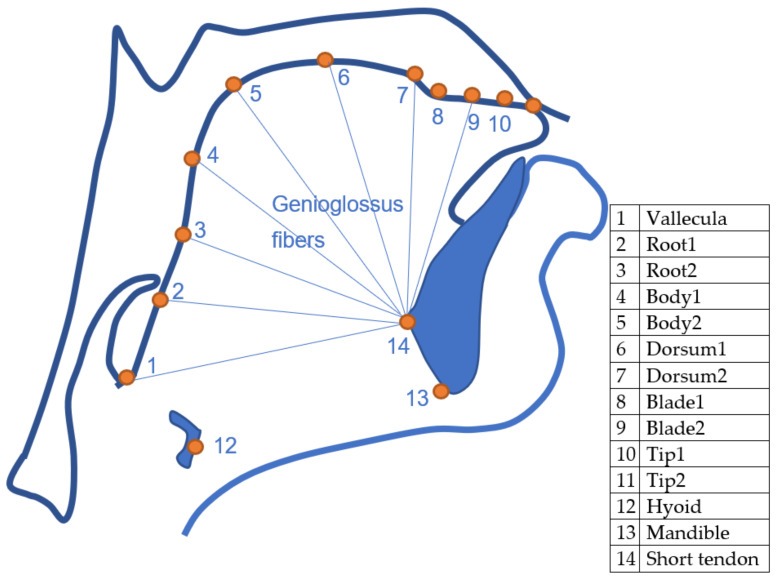
\includegraphics[keepaspectratio]{img/sensors-22-01133-g002.jpg}}

}

\caption{\label{fig-knots}Schematic representation of the knots tracked
by DeepLabCut. CC-BY Wrench and Balch-Tomes (Wrench 2024).}

\end{figure}%

Classical ways to analyse tongue contour data obtained from a fan-line
system, like SS-ANOVA (Davidson 2006; Chen and Lin 2011) and Generalised
Additive Models using polar coordinates (Coretta 2018b, n.d.), are not
appropriate with DLC tracked data due to the tongue contour ``curling''
onto itself along the root. This is illustrated in
Figure~\ref{fig-curl}: the plot shows the DLC tracked points (in black)
of the data from a Polish speaker and the traced tongue contours based
on the points (see Section~\ref{sec-gam-vc-coart} for details on the
data). The contours clearly curl onto themselves along the root (on the
left of the contour). The red smooths represent a LOESS smooth
calculated for Y along X: clearly this approach clearly miscalculates
the smooth for the back half of the tongue, simply because of the same X
value there are two Y values and the procedure returns something like an
average of the two values. Generalised Additive Models (introduced in
the following section) work on the same principle and hence would
produce the same type of error. Using polar coordinates would not solve
the problem: while a fan-line system lends itself easily to using polar
coordinates (since the origin of the probe can be used to approximate
the origin of the coordinate system), this can not be done with DLC data
because there is in reality no single origin in the actual tongue
anatomy from which vectors of displacement radiate that would work for
all tracked points.

\phantomsection\label{cell-fig-curl}
\begin{figure}[H]

\centering{

\pandocbounded{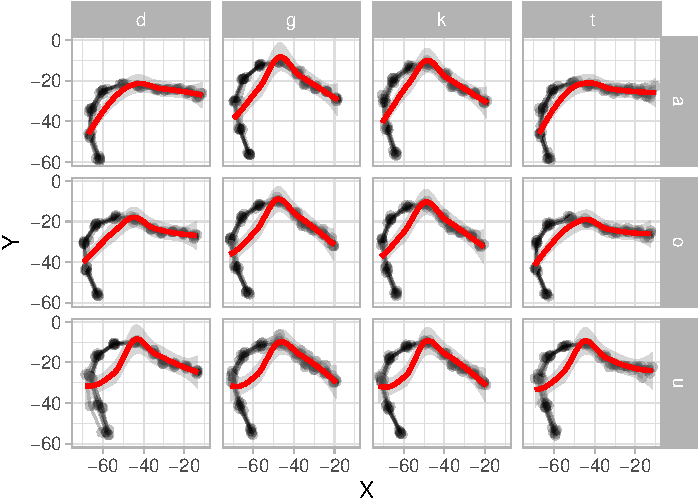
\includegraphics[keepaspectratio]{index_files/figure-pdf/fig-curl-1.pdf}}

}

\caption{\label{fig-curl}Illustrating tongue contours curling up along
the root. The estimated smooths in red fail to capture the curl.}

\end{figure}%

\textsubscript{Source:
\href{https://stefanocoretta.github.io/mv_uti/index.qmd.html}{Article
Notebook}}

In this tutorial, we introduce two alternative methods to analyse
DLC-tracked tongue contour data: Multivariate Generalised Additive
Models (Section~\ref{sec-gam}) and Multivariate Functional Principal
Component Analysis (Section~\ref{sec-fpca}). We will present the pros
and cons of each method in \textbf{?@sec-procons}, but to summarise we
are inclined to recommend Multivariate Functional Principal Component
Analysis over Multivariate Generalised Additive Models due to the
substantial computational overhead and reduced practical utility of the
latter over the former.

\section{Multivariate Generalised Additive Models}\label{sec-gam}

Generalised additive models (GAMs) are an extension of generalised
models that allow flexible modelling of non-linear effects (Hastie and
Tibshirani 1986; Wood 2006). GAMs are built upon smoothing splines
functions, the components of which are multiplied by estimated
coefficients to reconstruct an arbitrary time-changing curve. For a
thorough introduction to GAMs we refer the reader to (Sóskuthy 2021b,
2021a; Pedersen et al. 2019; Wieling 2018).

The data tracked by DeepLabCut consists of the position on the
horizontal (\emph{x}) and vertical (\emph{y}) axes of the fourteen
knots. In this tutorial, we will focus on modelling the tongue contour
based on the 11 knots from the vallecula to the tongue tip.
Figure~\ref{fig-tongue} illustrates the reconstructed tongue contour on
the basis of the 11 knots: the shown tongue is from the offset of a
vowel {[}o{]} followed by {[}t{]}, uttered by a Polish speaker (see
Section~\ref{sec-gam-vc-coart}).

\phantomsection\label{cell-fig-tongue}
\begin{figure}[H]

\centering{

\pandocbounded{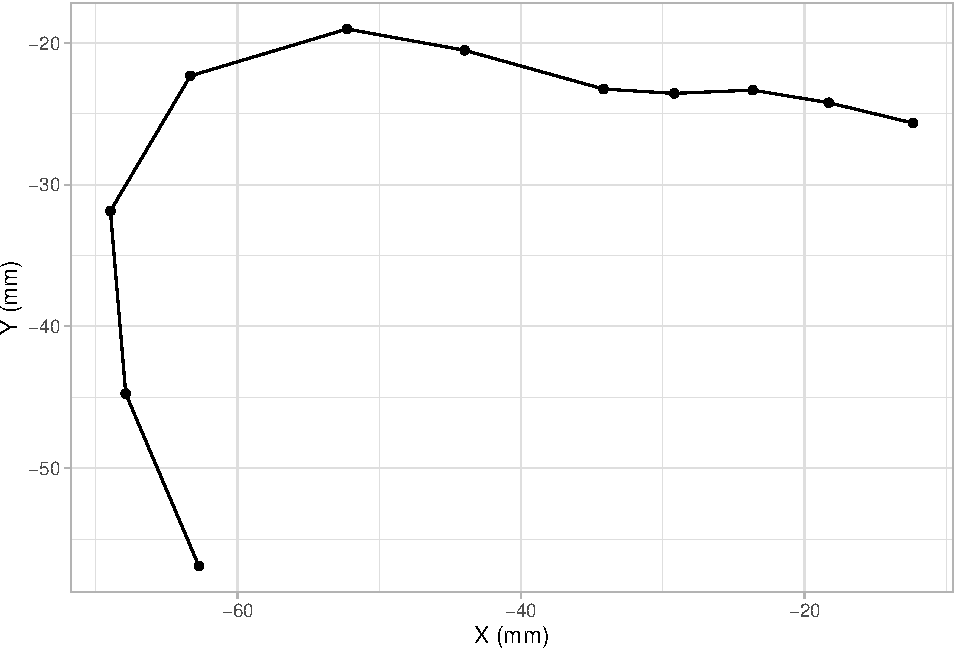
\includegraphics[keepaspectratio]{index_files/figure-pdf/fig-tongue-1.pdf}}

}

\caption{\label{fig-tongue}The eleven knots on the tongue contour taken
from the offset of {[}o{]} followed by {[}t{]} (Polish speaker PL04,
tongue tip to the right).}

\end{figure}%

\textsubscript{Source:
\href{https://stefanocoretta.github.io/mv_uti/index.qmd.html}{Article
Notebook}}

The same data is shown in Figure~\ref{fig-tongue-xy}, but in a different
format. Instead of a Cartesian coordinate system of X and Y values, the
plot has knot number on the \emph{x}-axis and X/Y coordinates on the
\emph{y}-axis. The X/Y coordinates thus form ``trajectories'' along the
knots. These trajectories are the ones that can be modelled using GAMs
and Functional Principal Component Analysis (FPCA). In this section, we
will illustrate GAMs applied to the X/Y trajectories along the knots and
how we can reconstruct the tongue contour from the modelled
trajectories. We will use data from two case studies of coarticulation:
vowel consonant (VC) coarticulation based on C place in Italian and
Polish, and consonantal articulation of plain vs emphatic consonants in
Lebanese Arabic.

\phantomsection\label{cell-fig-tongue-xy}
\begin{figure}[H]

\centering{

\pandocbounded{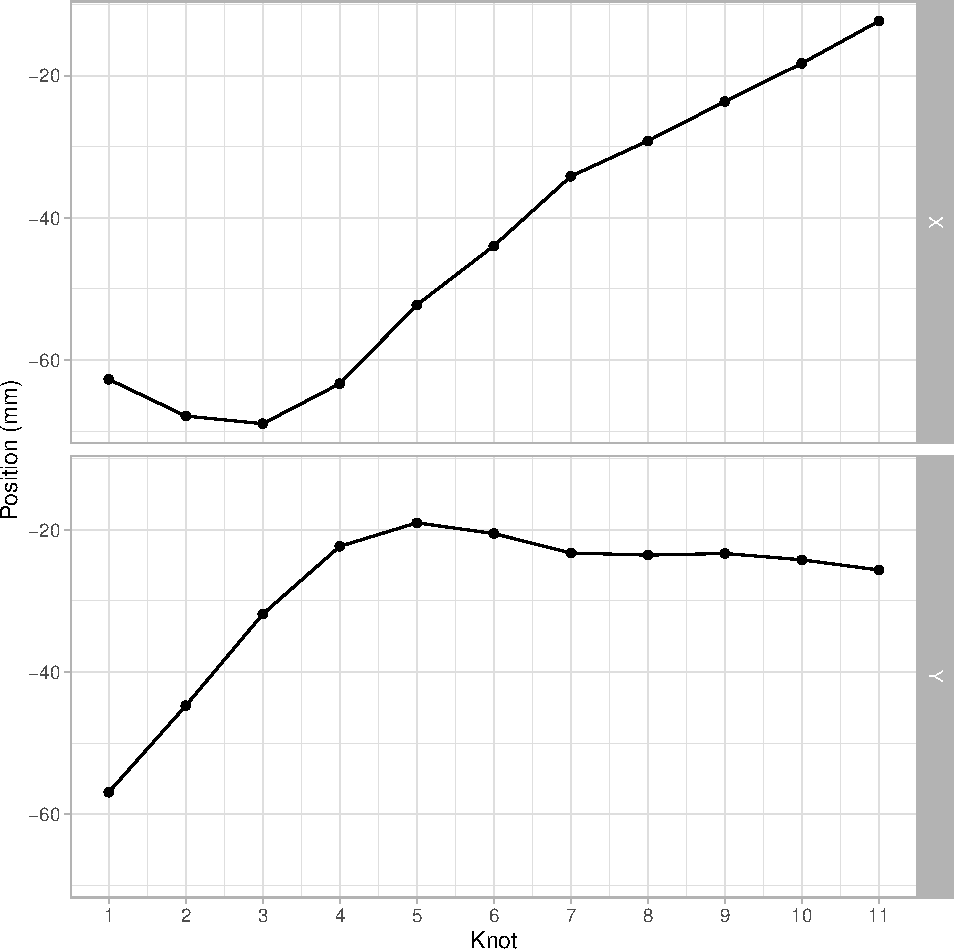
\includegraphics[keepaspectratio]{index_files/figure-pdf/fig-tongue-xy-1.pdf}}

}

\caption{\label{fig-tongue-xy}The horizontal and vertical positions of
the elevel knots (same data as Figure~\ref{fig-tongue}).}

\end{figure}%

\textsubscript{Source:
\href{https://stefanocoretta.github.io/mv_uti/index.qmd.html}{Article
Notebook}}

\subsection{VC coarticulation}\label{sec-gam-vc-coart}

The data of the first case study, Coretta (2018a), comes from Coretta
(2020b) and have been discussed in Coretta (2020a) (the analysis
concerned the position of the tongue root during the duration of vowels
followed by voiceless or voiced stops; in this paper we focus on tongue
contours at the vowel offset). The materials are /pVCV/ words embedded
in a frame sentence (\emph{Dico X lentamente} `I say X slowly' in
Italian and \emph{Mówię X teraz} `I say X now' in Polish). In the /pVCV/
words, C was /t, d, k, ɡ/ and V was /a, o, u/ (in each word, the two
vowels where identical, so for example \emph{pata, poto, putu}). The
data analysed here is from 9 speakers of Italian and 6 speakers of
Polish (other speakers were not included due to the difficulty in
processing their data with DeepLabCut).

Ultrasound tongue imaging was obtained with the set up by Articulate
Assistant Advanced™ (AAA, Ltd 2011). Spline data was extracted using a
custom DeepLabCut (DLC) model developed by Wrench and Balch-Tomes
(2022). When exporting from AAA™, the data was rotated based on the bite
plane, obtained with the imaging of a bite plate (Scobbie et al. 2011),
so that the bite plane is horizontal: this allows for a common
coordinate system where vertical and horizontal movement are comparable
across speakers. Once the DLC data was imported in R, we manually
removed tracking errors and we calculated \emph{z}-scores within each
speaker (the difference between the value and the mean, divided by the
standard deviation). These steps are documented in the paper's notebook
\href{notebooks/01_prepare_data.qmd}{Prepare data}.

The following code chunk reads the filtered data. A sample of the data
is shown in Table~\ref{tbl-dlc-voff}. Figure~\ref{fig-voff} shows the
tongue contours for each individual speaker. It is possible to notice
clusters of different contours, related to each of the vowels /a, o, u/.
Figure~\ref{fig-pl04} zooms in on PL04 (Polish): the contours of each
vowel are coloured separately, and two panels separate tongue contours
taken at the offset of vowels followed by coronal (/t, d/) and velar
stops (/k, ɡ/). Crucially, the variation in tongue shape at vowel offset
(or closure onset) across vowels contexts is higher in the coronal than
in the velar contexts. This is not surprising, giving the greater
involvement of the tongue body and dorsum (the relevant articulators of
vowel production) in velar than in coronal stops.

\begin{Shaded}
\begin{Highlighting}[]
\NormalTok{dlc\_voff\_f }\OtherTok{\textless{}{-}} \FunctionTok{readRDS}\NormalTok{(}\StringTok{"data/coretta2018/dlc\_voff\_f.rds"}\NormalTok{)}
\end{Highlighting}
\end{Shaded}

\textsubscript{Source:
\href{https://stefanocoretta.github.io/mv_uti/index.qmd.html}{Article
Notebook}}

\begin{longtable}[]{@{}llrrrl@{}}

\caption{\label{tbl-dlc-voff}A sample of the VC coarticulation data from
Coretta (2018a).}

\tabularnewline

\toprule\noalign{}
speaker & word & X & Y & knot & knot\_label \\
\midrule\noalign{}
\endhead
\bottomrule\noalign{}
\endlastfoot
it01 & pugu & -55.2105 & -44.1224 & 0 & Vallecula \\
it01 & pugu & -60.6994 & -31.3486 & 1 & Root\_1 \\
it01 & pugu & -65.1434 & -17.7311 & 2 & Root\_2 \\
it01 & pugu & -63.6757 & -4.2022 & 3 & Body\_1 \\
it01 & pugu & -57.2505 & 7.8483 & 4 & Body\_2 \\
it01 & pugu & -44.9086 & 13.3162 & 5 & Dorsum\_1 \\

\end{longtable}

\textsubscript{Source:
\href{https://stefanocoretta.github.io/mv_uti/index.qmd.html}{Article
Notebook}}

\phantomsection\label{cell-fig-voff}
\begin{figure}[H]

\centering{

\pandocbounded{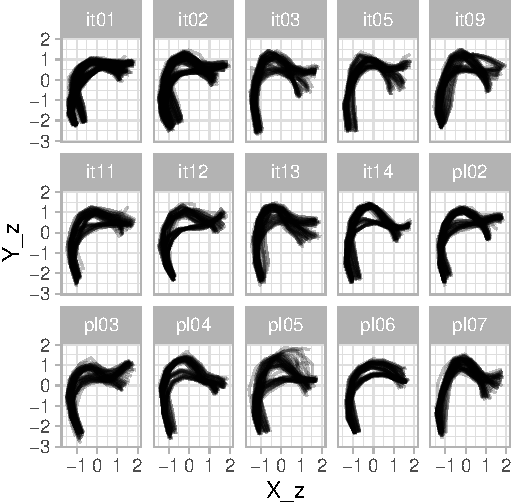
\includegraphics[keepaspectratio]{index_files/figure-pdf/fig-voff-1.pdf}}

}

\caption{\label{fig-voff}Tongue contours of 9 Italian speakers and6
Polish speakers, taken from the offset of the first vowel in /pCVCV/
target words.}

\end{figure}%

\textsubscript{Source:
\href{https://stefanocoretta.github.io/mv_uti/index.qmd.html}{Article
Notebook}}

\phantomsection\label{cell-fig-pl04}
\begin{figure}[H]

\centering{

\pandocbounded{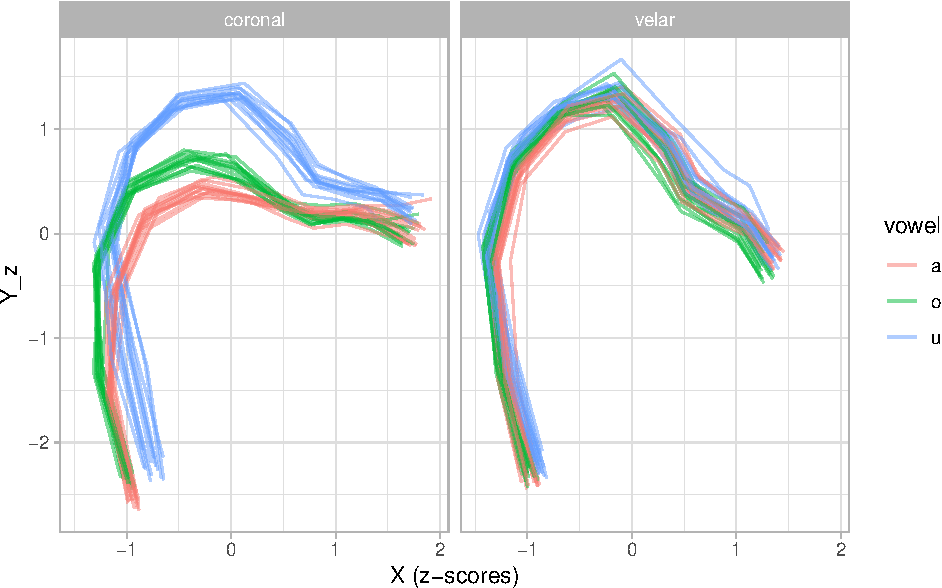
\includegraphics[keepaspectratio]{index_files/figure-pdf/fig-pl04-1.pdf}}

}

\caption{\label{fig-pl04}Tongue contours of PL04 (Polish) taken from the
offset of vowels followed by coronal or velar stops. Tip is on the
right.}

\end{figure}%

\textsubscript{Source:
\href{https://stefanocoretta.github.io/mv_uti/index.qmd.html}{Article
Notebook}}

We can now run a multivariate GAM to model the tongue contours. A
multivariate GAM can be fitted by providing model formulae for each
outcome variable (in our case, \texttt{X\_z} and \texttt{Y\_z}) in a
list. For example
\texttt{list(y\ \textasciitilde{}\ s(x),\ w\ \textasciitilde{}\ s(x))}
would instruct \texttt{mgcv::gam()} to fit a bivariate GAM with the two
outcome variables \texttt{y} and \texttt{w}. The required family is
\texttt{mvn} for ``multivariate normal'': \texttt{mvn(d\ =\ 2)}
indicates a bivariate family (a multivariate family with two dimensions,
i.e.~two outcome variables). In the model below, we are fitting a
multivariate GAM to the \emph{z}-scored X and Y coordinates. For both
outcome variables, we include a smooth over knot
(\texttt{s(knot,\ ...)}) with a \texttt{by} variable
\texttt{vow\_place\_lang}: this variable is built from an interaction of
vowel, place and language. (XXX note on categorical interactions in
GAMs). We set \texttt{k} to 5: this will usually be sufficient for X/Y
coordinates of tongue contours, since they are by nature not very
``wiggly'' (which would require a higher \texttt{k}). We also include a
factor smooth over knot for speaker (the equivalent of a non-linear
random effect) with \texttt{s(knot,\ speaker,\ ...)}: since language is
a between-speaker variable, we use \texttt{vow\_place} as the
\texttt{by} variable (\texttt{vow\_place} is the interaction of vowel
and place).

\begin{Shaded}
\begin{Highlighting}[]
\FunctionTok{library}\NormalTok{(mgcv)}

\NormalTok{voff\_gam }\OtherTok{\textless{}{-}} \FunctionTok{gam}\NormalTok{(}
  \FunctionTok{list}\NormalTok{(}
\NormalTok{    X\_z }\SpecialCharTok{\textasciitilde{}}\NormalTok{ vow\_place\_lang }\SpecialCharTok{+}
      \FunctionTok{s}\NormalTok{(knot, }\AttributeTok{by =}\NormalTok{ vow\_place\_lang, }\AttributeTok{k =} \DecValTok{5}\NormalTok{) }\SpecialCharTok{+}
      \FunctionTok{s}\NormalTok{(knot, speaker, }\AttributeTok{by =}\NormalTok{ vow\_place, }\AttributeTok{bs =} \StringTok{"fs"}\NormalTok{, }\AttributeTok{m =} \DecValTok{1}\NormalTok{),}
\NormalTok{    Y\_z }\SpecialCharTok{\textasciitilde{}}\NormalTok{ vow\_place\_lang }\SpecialCharTok{+}
      \FunctionTok{s}\NormalTok{(knot, }\AttributeTok{by =}\NormalTok{ vow\_place\_lang, }\AttributeTok{k =} \DecValTok{5}\NormalTok{) }\SpecialCharTok{+}
      \FunctionTok{s}\NormalTok{(knot, speaker, }\AttributeTok{by =}\NormalTok{ vow\_place, }\AttributeTok{bs =} \StringTok{"fs"}\NormalTok{, }\AttributeTok{m =} \DecValTok{1}\NormalTok{)}
\NormalTok{  ),}
  \AttributeTok{data =}\NormalTok{ dlc\_voff\_f,}
  \AttributeTok{family =} \FunctionTok{mvn}\NormalTok{(}\AttributeTok{d =} \DecValTok{2}\NormalTok{)}
\NormalTok{)}
\end{Highlighting}
\end{Shaded}

\textsubscript{Source:
\href{https://stefanocoretta.github.io/mv_uti/index.qmd.html}{Article
Notebook}}

The model summary is not particular insightful. What we are normally
interested in is the reconstructed tongue contours and in which
locations they are similar of different across conditions. To the best
of our knowledge, there isn't a straightforward way to compute sensible
measures of comparison, given the multidimensional nature of the model
(i.e., only one or the other outcome can be inspected at a time;
moreover, difference smooths, like in Sóskuthy (2021b) and Wieling
(2018), represent the difference of the \emph{sum} of the outcome
variables, rather than each outcome separately, Michele Gubian pers.
comm.) We thus recommend to plot the predicted tongue contours and base
any further inference on impressionistic observations on such predicted
contours. Alas, there is also no straightforward way to plot predicted
tongue contours, but to extract the predictions following a step-by-step
procedure, like the one illustrated in the following paragraphs.

First off, one has to create a grid of predictor values to obtain
predictions for. We do this with \texttt{expand\_grid()} in the
following code chunk. We start with unique values of \texttt{speaker},
\texttt{vow\_place} and \texttt{knot} (rather than just using integers
for the knots, we predict along increments of 0.1 from 0 to 10 for a
more refined tongue contour). We then create the required column
\texttt{vow\_place\_lang} by appending the language name based on the
speaker ID. Note that all variables included as predictors in the model
must be included in the prediction grid.

\begin{Shaded}
\begin{Highlighting}[]
\CommentTok{\# Create a grid of values to predict for}
\NormalTok{frame\_voff }\OtherTok{\textless{}{-}} \FunctionTok{expand\_grid}\NormalTok{(}
  \CommentTok{\# All the speakers}
  \AttributeTok{speaker =} \FunctionTok{unique}\NormalTok{(dlc\_voff\_f}\SpecialCharTok{$}\NormalTok{speaker),}
  \CommentTok{\# All vowel/place combinations}
  \AttributeTok{vow\_place =} \FunctionTok{unique}\NormalTok{(dlc\_voff\_f}\SpecialCharTok{$}\NormalTok{vow\_place),}
  \CommentTok{\# Knots from 0 to 10 by increments of 0.1}
  \CommentTok{\# This gives us greater resolution along the tongue contour than just using 10 knots}
  \AttributeTok{knot =} \FunctionTok{seq}\NormalTok{(}\DecValTok{0}\NormalTok{, }\DecValTok{10}\NormalTok{, }\AttributeTok{by =} \FloatTok{0.1}\NormalTok{)}
\NormalTok{) }\SpecialCharTok{|\textgreater{}} 
  \FunctionTok{mutate}\NormalTok{(}
    \AttributeTok{vow\_place\_lang =} \FunctionTok{case\_when}\NormalTok{(}
      \FunctionTok{str\_detect}\NormalTok{(speaker, }\StringTok{"it"}\NormalTok{) }\SpecialCharTok{\textasciitilde{}} \FunctionTok{paste0}\NormalTok{(vow\_place, }\StringTok{".Italian"}\NormalTok{),}
      \FunctionTok{str\_detect}\NormalTok{(speaker, }\StringTok{"pl"}\NormalTok{) }\SpecialCharTok{\textasciitilde{}} \FunctionTok{paste0}\NormalTok{(vow\_place, }\StringTok{".Polish"}\NormalTok{)}
\NormalTok{    )}
\NormalTok{  )}
\end{Highlighting}
\end{Shaded}

\textsubscript{Source:
\href{https://stefanocoretta.github.io/mv_uti/index.qmd.html}{Article
Notebook}}

With the prediction grid \texttt{frame\_voff} we can now extract
predictions from the model \texttt{voff\_gam} with \texttt{predict()}.
This function requires the GAM model object (\texttt{voff\_gam}) and the
prediction grid (\texttt{frame\_off}). We also obtain the standard error
of the prediction which we will use to calculate Confidence Intervals in
the next step. Since we have used factor smooths for speaker, we now
have to manually exclude these smooths from the prediction to obtain a
``population'' level prediction. We do this by listing the smooths to be
removed in \texttt{excl}: note that the smooths must be named as they
are in the summary of the model, so always check the summary to ensure
you list all of the factor smooths. Finally, we rename the columns with
the name of the outcome variables.

\begin{Shaded}
\begin{Highlighting}[]
\CommentTok{\# List of factor smooths, to be excluded from prediction}
\NormalTok{excl }\OtherTok{\textless{}{-}} \FunctionTok{c}\NormalTok{(}
  \StringTok{"s(knot,speaker):vow\_placea.coronal"}\NormalTok{,}
  \StringTok{"s(knot,speaker):vow\_placeo.coronal"}\NormalTok{,}
  \StringTok{"s(knot,speaker):vow\_placeu.coronal"}\NormalTok{,}
  \StringTok{"s(knot,speaker):vow\_placea.velar"}\NormalTok{,}
  \StringTok{"s(knot,speaker):vow\_placeo.velar"}\NormalTok{,}
  \StringTok{"s(knot,speaker):vow\_placeu.velar"}\NormalTok{,}
  \StringTok{"s.1(knot,speaker):vow\_placea.coronal"}\NormalTok{,}
  \StringTok{"s.1(knot,speaker):vow\_placeo.coronal"}\NormalTok{,}
  \StringTok{"s.1(knot,speaker):vow\_placeu.coronal"}\NormalTok{,}
  \StringTok{"s.1(knot,speaker):vow\_placea.velar"}\NormalTok{,}
  \StringTok{"s.1(knot,speaker):vow\_placeo.velar"}\NormalTok{,}
  \StringTok{"s.1(knot,speaker):vow\_placeu.velar"}
\NormalTok{)}

\CommentTok{\# Get prediction from model voff\_gam}
\NormalTok{voff\_gam\_p }\OtherTok{\textless{}{-}} \FunctionTok{predict}\NormalTok{(voff\_gam, frame\_voff, }\AttributeTok{se.fit =} \ConstantTok{TRUE}\NormalTok{, }\AttributeTok{exclude =}\NormalTok{ excl) }\SpecialCharTok{|\textgreater{}}
  \FunctionTok{as.data.frame}\NormalTok{() }\SpecialCharTok{|\textgreater{}}
  \FunctionTok{as\_tibble}\NormalTok{()}

\CommentTok{\# Rename columns}
\FunctionTok{colnames}\NormalTok{(voff\_gam\_p) }\OtherTok{\textless{}{-}} \FunctionTok{c}\NormalTok{(}\StringTok{"X"}\NormalTok{, }\StringTok{"Y"}\NormalTok{, }\StringTok{"X\_se"}\NormalTok{, }\StringTok{"Y\_se"}\NormalTok{)}
\end{Highlighting}
\end{Shaded}

\textsubscript{Source:
\href{https://stefanocoretta.github.io/mv_uti/index.qmd.html}{Article
Notebook}}

Now we have to join the prediction in \texttt{voff\_gam\_p} with the
prediction frame, so that we have all the predictor values in the same
data frame. We do so here with \texttt{bind\_cols()} from the dplyr
package. Note that \texttt{voff\_gam\_p} contains predictions for each
level of the factor smooths, despite these being excluded from
prediction. If you inspect the predictions for different speakers, you
will find that they are the same for the same levels of
\texttt{vow\_place\_lang}: this is because the effects of the factor
smooths were removed, so \texttt{speaker} has no effect on the predicted
values. This means that you can pick any Italian and Polish speaker in
the predicted data frame. We do so by filtering with
\texttt{filter(speaker\ \%in\%\ c("it01",\ "pl02"))}, but any other
speaker would lead to the same output. We also calculate the lower and
upper limits of 95\% Confidence intervals (CI) for each coordinate. Note
that you should interpret these CI with a grain of salt, because they
are not truly multivariate, but rather represent the CI on each
coordinate axis independently.

\begin{Shaded}
\begin{Highlighting}[]
\NormalTok{voff\_gam\_p }\OtherTok{\textless{}{-}} \FunctionTok{bind\_cols}\NormalTok{(frame\_voff, voff\_gam\_p) }\SpecialCharTok{|\textgreater{}} 
  \CommentTok{\# pick any Italian and Polish speaker, random effects have been removed}
  \FunctionTok{filter}\NormalTok{(speaker }\SpecialCharTok{\%in\%} \FunctionTok{c}\NormalTok{(}\StringTok{"it01"}\NormalTok{, }\StringTok{"pl02"}\NormalTok{)) }\SpecialCharTok{|\textgreater{}} 
  \CommentTok{\# Calculate 95\% CIs of X and Y}
  \FunctionTok{mutate}\NormalTok{(}
    \AttributeTok{X\_lo =}\NormalTok{ X }\SpecialCharTok{{-}}\NormalTok{ (}\FloatTok{1.96} \SpecialCharTok{*}\NormalTok{ X\_se),}
    \AttributeTok{X\_hi =}\NormalTok{ X }\SpecialCharTok{+}\NormalTok{ (}\FloatTok{1.96} \SpecialCharTok{*}\NormalTok{ X\_se),}
    \AttributeTok{Y\_lo =}\NormalTok{ Y }\SpecialCharTok{{-}}\NormalTok{ (}\FloatTok{1.96} \SpecialCharTok{*}\NormalTok{ Y\_se),}
    \AttributeTok{Y\_hi =}\NormalTok{ Y }\SpecialCharTok{+}\NormalTok{ (}\FloatTok{1.96} \SpecialCharTok{*}\NormalTok{ Y\_se)}
\NormalTok{  ) }\SpecialCharTok{|\textgreater{}} 
  \CommentTok{\# Separate column into individual variables, for plotting later}
  \FunctionTok{separate}\NormalTok{(vow\_place\_lang, }\FunctionTok{c}\NormalTok{(}\StringTok{"vowel"}\NormalTok{, }\StringTok{"place"}\NormalTok{, }\StringTok{"language"}\NormalTok{))}
\end{Highlighting}
\end{Shaded}

\textsubscript{Source:
\href{https://stefanocoretta.github.io/mv_uti/index.qmd.html}{Article
Notebook}}

Figure~\ref{fig-voff-pred} and Figure~\ref{fig-voff-ci} show the
predicted tongue contours based on the \texttt{voff\_gam} model, without
and with 95\% CIs respectively. As mentioned earlier, there isn't a
straightforward way to obtain any statistical measure of the difference
between the contours on the multivariate plane, so we must be content
with the figure.

\phantomsection\label{cell-fig-voff-pred}
\begin{figure}[H]

\centering{

\pandocbounded{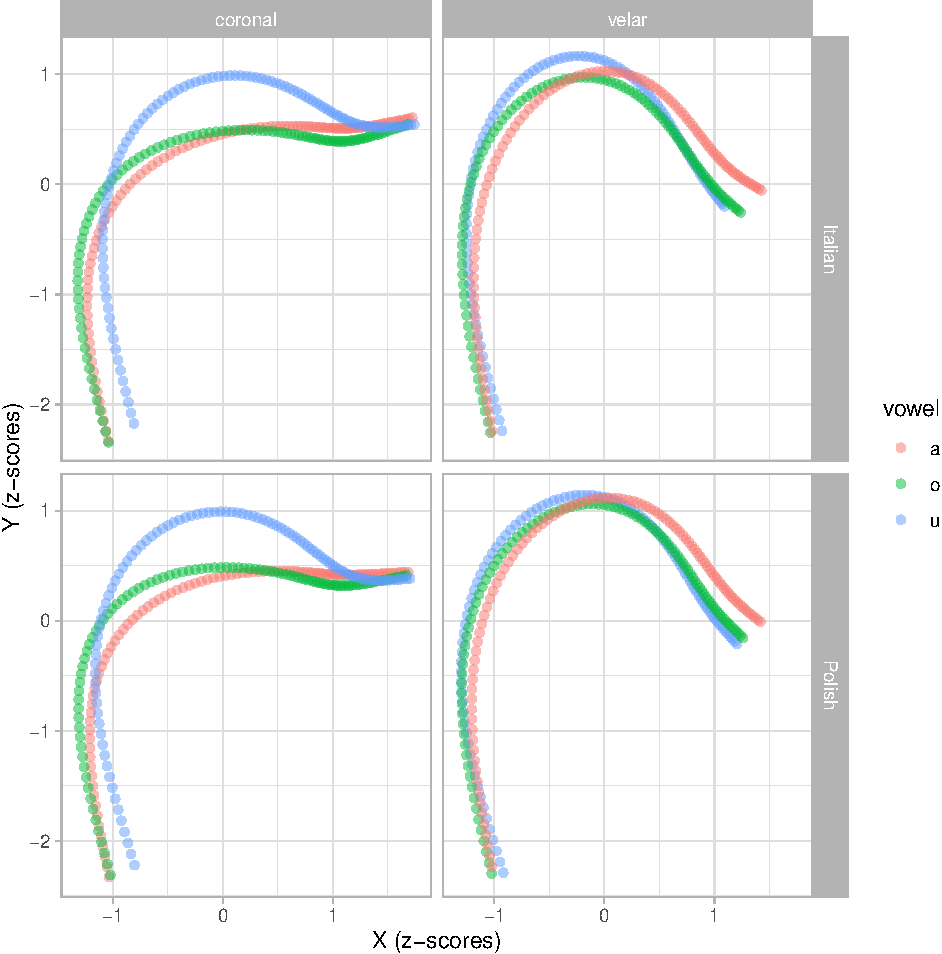
\includegraphics[keepaspectratio]{index_files/figure-pdf/fig-voff-pred-1.pdf}}

}

\caption{\label{fig-voff-pred}Predicted tongue contours based on a
multivariate GAM. Uncertainty not shown.}

\end{figure}%

\textsubscript{Source:
\href{https://stefanocoretta.github.io/mv_uti/index.qmd.html}{Article
Notebook}}

\phantomsection\label{cell-fig-voff-ci}
\begin{figure}[H]

\centering{

\pandocbounded{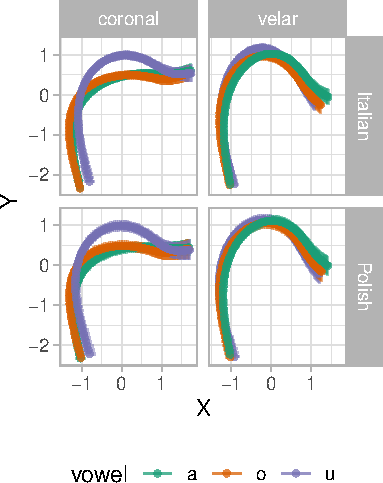
\includegraphics[keepaspectratio]{index_files/figure-pdf/fig-voff-ci-1.pdf}}

}

\caption{\label{fig-voff-ci}Predicted tongue contours based on a
multivariate GAM, with 95\% Confidence Intervals.}

\end{figure}%

\textsubscript{Source:
\href{https://stefanocoretta.github.io/mv_uti/index.qmd.html}{Article
Notebook}}

\subsection{Emphaticness}\label{emphaticness}

\begin{Shaded}
\begin{Highlighting}[]
\NormalTok{dlc\_emph\_f }\OtherTok{\textless{}{-}} \FunctionTok{readRDS}\NormalTok{(}\StringTok{"data/sakr2025/dlc\_emph\_f.rds"}\NormalTok{)}
\end{Highlighting}
\end{Shaded}

\textsubscript{Source:
\href{https://stefanocoretta.github.io/mv_uti/index.qmd.html}{Article
Notebook}}

\textsubscript{Source:
\href{https://stefanocoretta.github.io/mv_uti/index.qmd.html}{Article
Notebook}}

\textsubscript{Source:
\href{https://stefanocoretta.github.io/mv_uti/index.qmd.html}{Article
Notebook}}

\phantomsection\label{cell-fig-emph-pred}
\begin{figure}[H]

\centering{

\pandocbounded{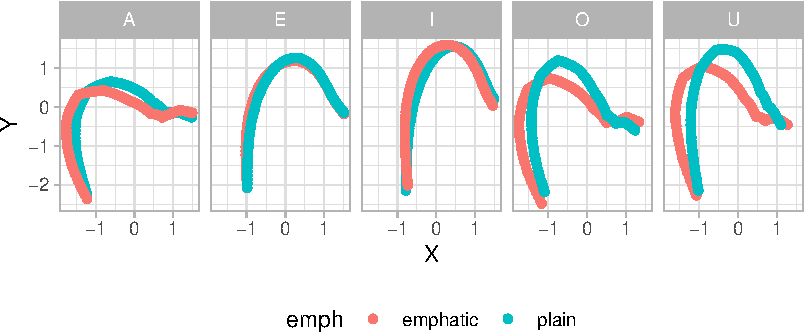
\includegraphics[keepaspectratio]{index_files/figure-pdf/fig-emph-pred-1.pdf}}

}

\caption{\label{fig-emph-pred}}

\end{figure}%

\textsubscript{Source:
\href{https://stefanocoretta.github.io/mv_uti/index.qmd.html}{Article
Notebook}}

\phantomsection\label{cell-fig-emph-ci}
\begin{figure}[H]

\centering{

\pandocbounded{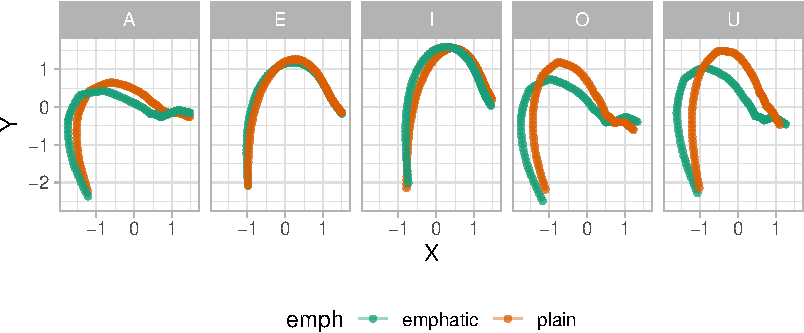
\includegraphics[keepaspectratio]{index_files/figure-pdf/fig-emph-ci-1.pdf}}

}

\caption{\label{fig-emph-ci}}

\end{figure}%

\textsubscript{Source:
\href{https://stefanocoretta.github.io/mv_uti/index.qmd.html}{Article
Notebook}}

\textsubscript{Source:
\href{https://stefanocoretta.github.io/mv_uti/index.qmd.html}{Article
Notebook}}

\phantomsection\label{cell-fig-emph-part}
\begin{figure}[H]

\centering{

\pandocbounded{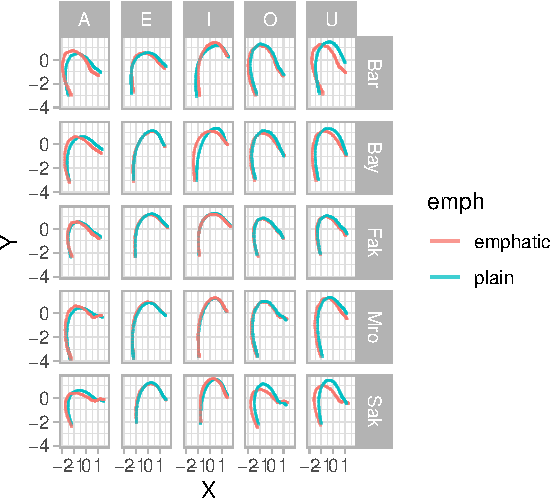
\includegraphics[keepaspectratio]{index_files/figure-pdf/fig-emph-part-1.pdf}}

}

\caption{\label{fig-emph-part}}

\end{figure}%

\textsubscript{Source:
\href{https://stefanocoretta.github.io/mv_uti/index.qmd.html}{Article
Notebook}}

\section{Multivariate Functional Principal Component
Analysis}\label{sec-fpca}

\subsection{VC coarticulation}\label{vc-coarticulation}

We will apply Multivariate Functional Principal Component Analysis
(MFPCA). The following code has been adapted from Gubian (2024). The
packages below are needed to run MFPCA (except landmarkregUtils, they
are available on CRAN).

\textsubscript{Source:
\href{https://stefanocoretta.github.io/mv_uti/index.qmd.html}{Article
Notebook}}

The format required to work through MFPCA is a ``long'' format with one
column containing the coordinate labels (\emph{x} or \emph{y}
coordinate) and another with the coordinate values. We can easily pivot
the data with \texttt{pivot\_longer()}. Note that we are using the
\emph{z}-scored coordinate values (\texttt{X\_z} and \texttt{Y\_z}). If
you are not unsure about what the code in this section, it is always
useful to inspect intermediate and final output.

\textsubscript{Source:
\href{https://stefanocoretta.github.io/mv_uti/index.qmd.html}{Article
Notebook}}

In the second step, we create a \texttt{multiFunData} object: this is a
special type of list object, with the observations of the two
coordinates (\texttt{X\_z} and \texttt{Y\_z}) as two matrices of
dimension \(N \cdot 11\), where \(N\) is the number of tongue contours
and \(11\) is for the 11 knots returned by DLC. Three columns in the
data are used to create the \texttt{multiFunData} object: one column
with the id of each contour (in our data, \texttt{frame\_id}), a time or
series column (\texttt{knot}) and the column with the coordinate values
(\texttt{value}).

\textsubscript{Source:
\href{https://stefanocoretta.github.io/mv_uti/index.qmd.html}{Article
Notebook}}

Once we have our \texttt{multFunData} object, we can use the
\texttt{MFPCA()} function to compute an MFPCA. In this tutorial we will
compute the first two PCs, but you can compute up to \(K-1\) PCs where
\(K\) is the number of DLC knots in the data.

\textsubscript{Source:
\href{https://stefanocoretta.github.io/mv_uti/index.qmd.html}{Article
Notebook}}

We can quickly calculate the proportion of explained variance of each PC
with the following code. PC1 and PC2 together explain almost 100\% of
the variance in our data. The higher the variance explained, the better
the variance patterns in the data are captured.

\begin{verbatim}
[1] 0.7108713 0.2891287
\end{verbatim}

\textsubscript{Source:
\href{https://stefanocoretta.github.io/mv_uti/index.qmd.html}{Article
Notebook}}

The best way to assess the effect of the PC scores on the shape of the
tongue contours is to plot the predicted tongue contours based on a set
of representative PC scores. In order to be able to plot the predicted
contours, we need to calculate them from the MFPCA object. Gubian
suggests plotting predicted curves at score intervals based on fractions
of the scores standard deviation. This is what the following code does.

\textsubscript{Source:
\href{https://stefanocoretta.github.io/mv_uti/index.qmd.html}{Article
Notebook}}

The created data frame \texttt{pc\_curves} has the predicted values of
the X and Y coordinates \emph{along the knots}. This is the same
structure as Figure~\ref{fig-tongue-xy}, with the knot number on the
\emph{x}-axis and the coordinates on the \emph{y}-axis. Of course, what
we are after is the X/Y plot of the tongue contours, rather than the
knot/coordinate plot as needed to fit an MFPCA. For the sake of clarity,
we first plot the predicted curves for X and Y separately.
Figure~\ref{fig-pc-curves} shows these. The plot is composed of four
panels: the top two are the predicted curves along knot number for the Y
coordinates (based on PC1 in the left panel and PC2 in the right panel).
Interpreting the effect of the PCs on the X and Y coordinates separately
allows one to observe vertical (Y coordinate) and horizontal (X
coordinate) differences in tongue position independently. However, note
that the vector of muscle contractions in the tongue are not simply
along a vertical/horizontal axis (Honda 1996; Wrench 2024). Looking at a
full tongue contour (in an X/Y coordinates plot) will generally prove to
be more straightforward.

\phantomsection\label{cell-fig-pc-curves}
\begin{figure}[H]

\centering{

\pandocbounded{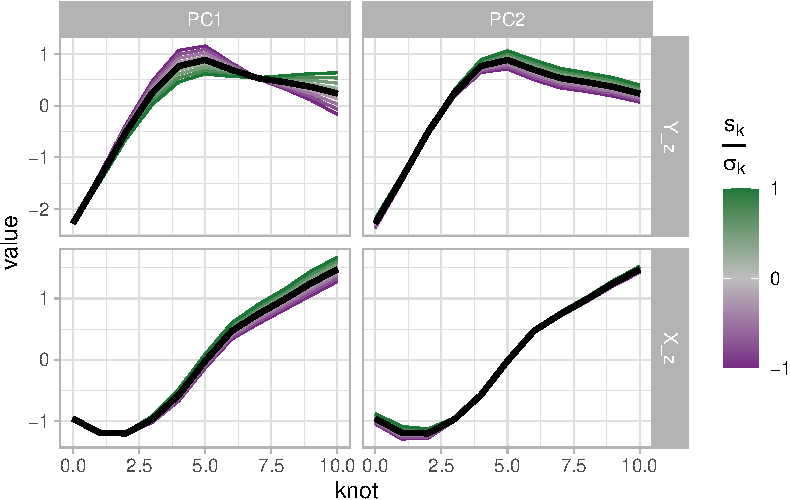
\includegraphics[keepaspectratio]{index_files/figure-pdf/fig-pc-curves-1.pdf}}

}

\caption{\label{fig-pc-curves}Predicted curves along knot number for X
and Y coordinates, as obtained from an MFPCA.}

\end{figure}%

\textsubscript{Source:
\href{https://stefanocoretta.github.io/mv_uti/index.qmd.html}{Article
Notebook}}

In order to plot tongue contours in the X/Y coordinate system, we simply
need to pivot the data to a wider format.

\textsubscript{Source:
\href{https://stefanocoretta.github.io/mv_uti/index.qmd.html}{Article
Notebook}}

Figure~\ref{fig-contours} plots the predicted contours based on the the
PC scores (specifically, fractions of the standard deviation of the PC
scores). The \emph{x} and \emph{y}-axes correspond to the X and Y
coordinates of the tongue contour, with the effect of PC1 in the left
panel and the effect of PC2 in the right panel. A higher PC1 score
(green lines in the left panel) suggest a lowering of the tongue
body/dorsum and raising of the tongue tip. Since the data contains velar
and coronal consonants, we take this to be capturing the velar/coronal
place of articulation effect. A higher PC2 score (green lines in the
right panel) corresponds to an overall higher tongue position.
Considering that the back/central vowels /a, o, u/ are included in this
data set, we take PC2 to be related with the effect of vowel on the
tongue shape at closure onset.

\phantomsection\label{cell-fig-contours}
\begin{figure}[H]

\centering{

\pandocbounded{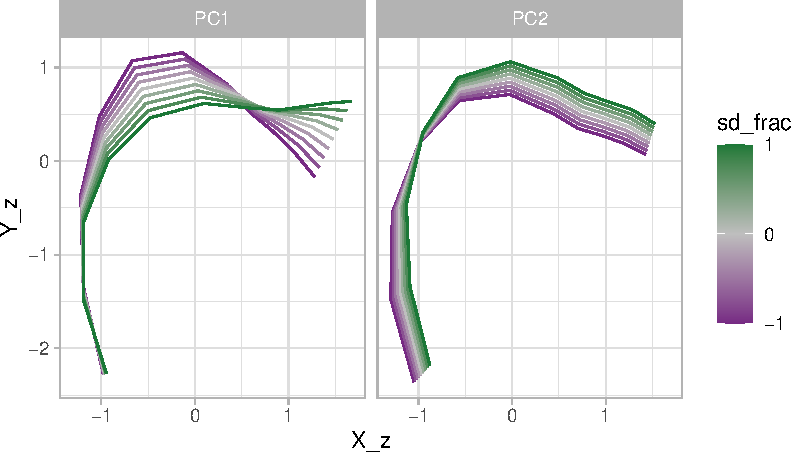
\includegraphics[keepaspectratio]{index_files/figure-pdf/fig-contours-1.pdf}}

}

\caption{\label{fig-contours}Predicted tongue contours as obtained from
an MFPCA.}

\end{figure}%

\textsubscript{Source:
\href{https://stefanocoretta.github.io/mv_uti/index.qmd.html}{Article
Notebook}}

Given the patterns in Figure~\ref{fig-contours}, we can expect to see
differences in PC2 scores based on the vowel if there is VC
coarticulation. We can obtain the PC scores of each observation in the
data with the following code.

\textsubscript{Source:
\href{https://stefanocoretta.github.io/mv_uti/index.qmd.html}{Article
Notebook}}

Figure~\ref{fig-pc-scores} plots PC scores by language (rows), consonant
place (columns) and vowel (colour). Both in Italian and Polish, we can
observe a clear coarticulatory effect of /u/ on the production of
coronal stops (and perhaps minor differences in /a/ vs /o/). On the
other hand, the effect of vowel in velar stops seems to be minimal,
again in both languages. This is not entirely surprising, since while
coronal stops allow for adjustments of (and coarticulatory effect on)
the tongue body, velar stops do not since it is precisely the tongue
body/dorsum that is raised to produce the velar closure.

\phantomsection\label{cell-fig-pc-scores}
\begin{figure}[H]

\centering{

\pandocbounded{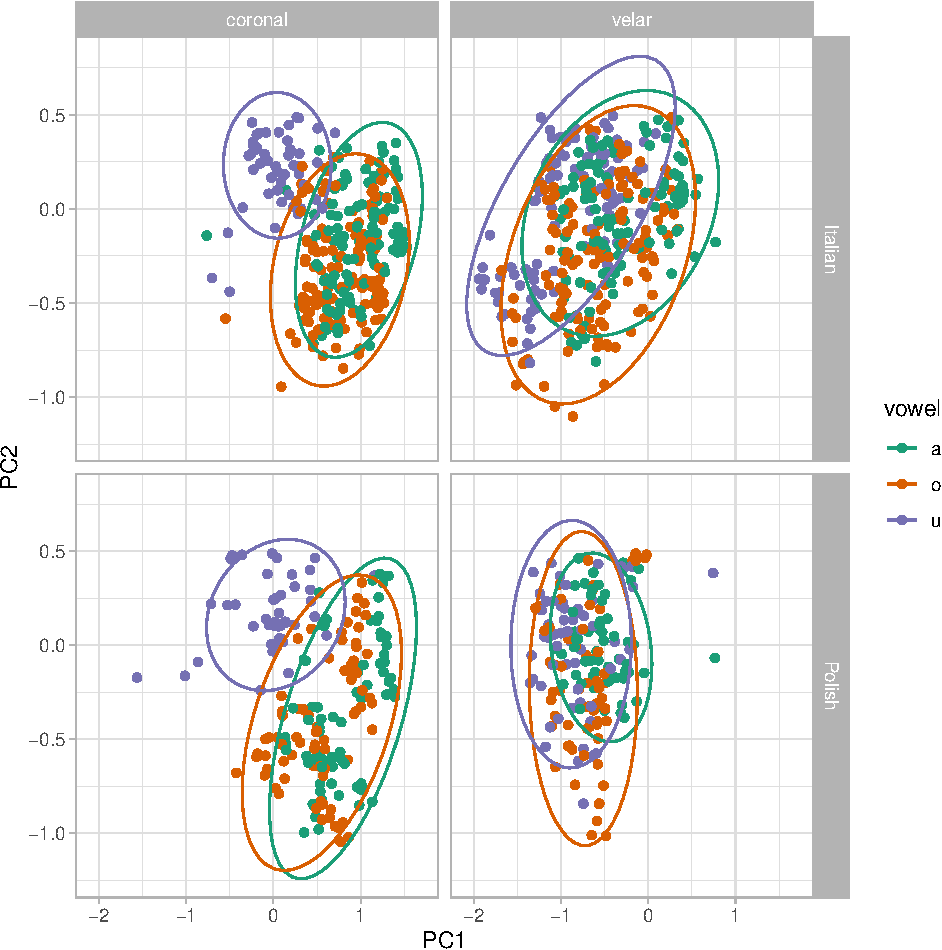
\includegraphics[keepaspectratio]{index_files/figure-pdf/fig-pc-scores-1.pdf}}

}

\caption{\label{fig-pc-scores}PC1/PC2 scores by language, consonant
place of articulation and vowel.}

\end{figure}%

\textsubscript{Source:
\href{https://stefanocoretta.github.io/mv_uti/index.qmd.html}{Article
Notebook}}

Once one has established which patterns each PC is capturing, PC scores
can be submitted to further statistical modelling, like for example
regression models where the PC scores are outcome variables and several
predictors are include to assess possible differences in PC scores.

\subsection{Emphaticness}\label{emphaticness-1}

In this section we will run an MFPCA analysis on the Lebanese Arabic
data. Since the procedure is the same as in the previous section, the
code will not be shown here, but can be viewed in the article notebook,
at XXX.

Figure~\ref{fig-emph-curves-wide} illustrates the reconstructed tongue
contours (taken from 35 ms before the CV boundary) in Lebanese Arabic,
based on the MFPCA. PC1 captures the low-back/high-front diagonal
movement. PC2, on the other hand, seems to be restricted to high/low
movement at the back of the oral cavity. Emphatic consonants, if
produced with a constricted pharynx (i.e.~paryngealised), should have a
lower PC1. If on the other hand they are produced with a raised tongue
dorsum (i.e.~velarised), they should have a lower PC2 (lower PC scores
are in purple in Figure~\ref{fig-emph-curves-wide}).

\phantomsection\label{cell-fig-emph-curves-wide}
\begin{figure}[H]

\centering{

\pandocbounded{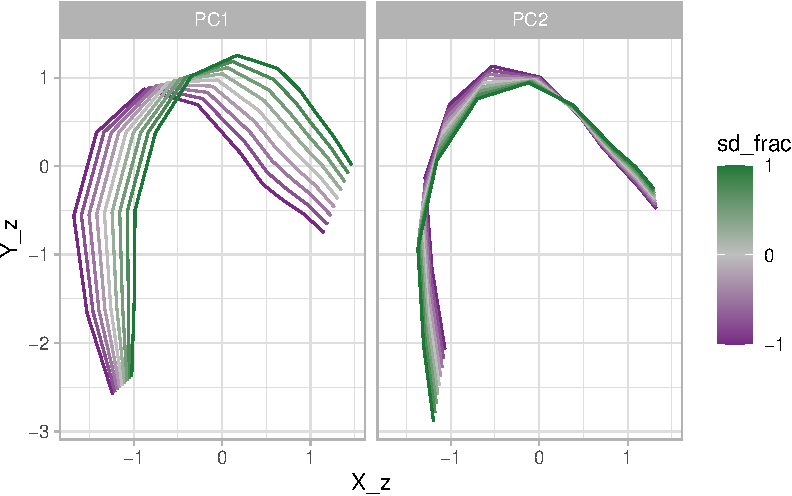
\includegraphics[keepaspectratio]{index_files/figure-pdf/fig-emph-curves-wide-1.pdf}}

}

\caption{\label{fig-emph-curves-wide}Predicted tongue contours of
Lebanese Arabic coronal consonants as obtained from an MFPCA.}

\end{figure}%

\textsubscript{Source:
\href{https://stefanocoretta.github.io/mv_uti/index.qmd.html}{Article
Notebook}}

\phantomsection\label{cell-fig-emph-speakers}
\begin{figure}[H]

\centering{

\pandocbounded{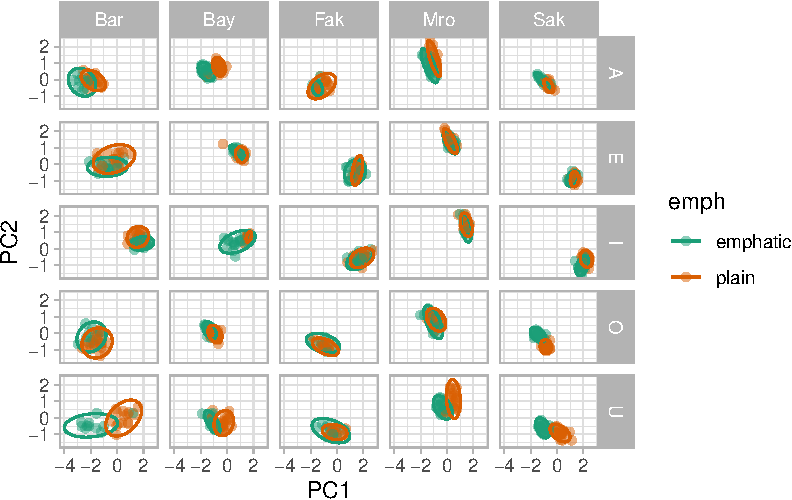
\includegraphics[keepaspectratio]{index_files/figure-pdf/fig-emph-speakers-1.pdf}}

}

\caption{\label{fig-emph-speakers}PC1 and PC2 scores by vowel, consonant
type and speaker.}

\end{figure}%

\textsubscript{Source:
\href{https://stefanocoretta.github.io/mv_uti/index.qmd.html}{Article
Notebook}}

\phantomsection\label{cell-fig-emph-pc1}
\begin{figure}[H]

\centering{

\pandocbounded{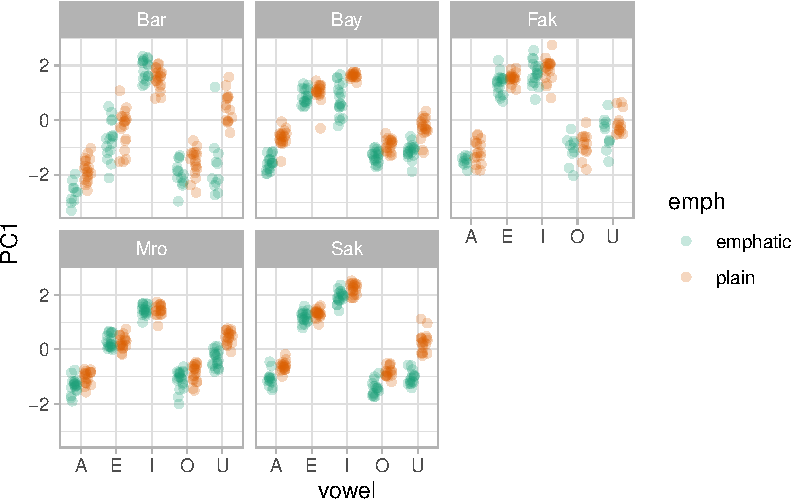
\includegraphics[keepaspectratio]{index_files/figure-pdf/fig-emph-pc1-1.pdf}}

}

\caption{\label{fig-emph-pc1}}

\end{figure}%

\textsubscript{Source:
\href{https://stefanocoretta.github.io/mv_uti/index.qmd.html}{Article
Notebook}}

\phantomsection\label{cell-fig-emph-pc2}
\begin{figure}[H]

\centering{

\pandocbounded{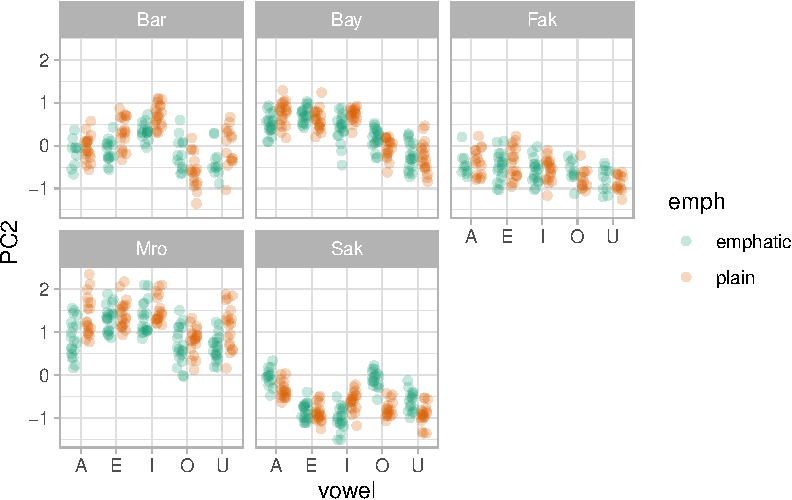
\includegraphics[keepaspectratio]{index_files/figure-pdf/fig-emph-pc2-1.pdf}}

}

\caption{\label{fig-emph-pc2}}

\end{figure}%

\textsubscript{Source:
\href{https://stefanocoretta.github.io/mv_uti/index.qmd.html}{Article
Notebook}}

\phantomsection\label{refs}
\begin{CSLReferences}{1}{0}
\bibitem[\citeproctext]{ref-chen2011}
Chen, Yu, and Hua Lin. 2011. {``Analysing Tongue Shape and Movement in
Vowel Production Using SS-ANOVA in Ultrasound Imaging.''} In, 1721.

\bibitem[\citeproctext]{ref-coretta2018f}
Coretta, Stefano. 2018a. {``An Exploratory Study of the Voicing Effect
in Italian and Polish {[}Data V1.0.0{]}.''}
\url{https://doi.org/10.17605/OSF.IO/8ZHKU}.

\bibitem[\citeproctext]{ref-coretta2018c}
---------. 2018b. {``Using Generalised Additive Models (GAM) with Polar
Coordinates for Assessing Tongue Contours.''}
\url{https://stefanocoretta.github.io/rticulate/articles/polar-gams.html}.

\bibitem[\citeproctext]{ref-coretta2020}
---------. 2020a. {``Longer Vowel Duration Correlates with Greater
Tongue Root Advancement at Vowel Offset: Acoustic and Articulatory Data
from Italian and Polish.''} \emph{The Journal of the Acoustical Society
of America} 147: 245259. \url{https://doi.org/10.1121/10.0000556}.

\bibitem[\citeproctext]{ref-coretta2020b}
---------. 2020b. {``Vowel Duration and Consonant Voicing: A Production
Study.''} PhD thesis.

\bibitem[\citeproctext]{ref-coretta2019g}
---------. n.d. {``Assessing Mid-Saggital Tongue Contours in Polar
Coordinates Using Generalised Additive (Mixed) Models.''}
\url{https://doi.org/10.31219/osf.io/q6vzb}.

\bibitem[\citeproctext]{ref-davidson2006}
Davidson, Lisa. 2006. {``Comparing Tongue Shapes from Ultrasound Imaging
Using Smoothing Spline Analysis of Variance.''} \emph{The Journal of the
Acoustical Society of America} 120 (1): 407415.
\url{https://doi.org/10.1121/1.2205133}.

\bibitem[\citeproctext]{ref-epstein2005}
Epstein, Melissa A., and Maureen Stone. 2005. {``The Tongue Stops Here:
Ultrasound Imaging of the Palate.''} \emph{The Journal of the Acoustical
Society of America} 118 (4): 21282131.
\url{https://doi.org/10.1121/1.2031977}.

\bibitem[\citeproctext]{ref-gubian2024}
Gubian, Michele. 2024. \emph{Workshop on Functional PCA for Phonetics
and Prosody}. \url{https://github.com/uasolo/FPCA-phonetics-workshop}.

\bibitem[\citeproctext]{ref-hastie1986}
Hastie, Trevor, and Robert Tibshirani. 1986. {``Generalized Additive
Models.''} \emph{Statistical Science} 1 (3): 297310.
\url{https://doi.org/10.1201/9780203753781-6}.

\bibitem[\citeproctext]{ref-honda1996}
Honda, Kiyoshi. 1996. {``Organization of Tongue Articulation for
Vowels.''} \emph{Journal of Phonetics} 24 (1): 3952.
\url{https://doi.org/10.1006/jpho.1996.0004}.

\bibitem[\citeproctext]{ref-ltd2011}
Ltd, Articulate Instruments. 2011. {``Articulate Assistant Advanced User
Guide. {Version} 2.16.''}

\bibitem[\citeproctext]{ref-lulich2018}
Lulich, Steven M., Kelly H. Berkson, and Kenneth de Jong. 2018.
{``Acquiring and Visualizing 3d/4d Ultrasound Recordings of Tongue
Motion.''} \emph{Journal of Phonetics} 71: 410424.
\url{https://doi.org/10.1016/j.wocn.2018.10.001}.

\bibitem[\citeproctext]{ref-pedersen2019}
Pedersen, Eric J., David L. Miller, Gavin L. Simpson, and Noam Ross.
2019. {``Hierarchical Generalized Additive Models in Ecology: An
Introduction with Mgcv.''} \emph{PeerJ} 7: e6876.
\url{https://doi.org/10.7717/peerj.6876}.

\bibitem[\citeproctext]{ref-scobbie2011}
Scobbie, James M., Eleanor Lawson, Steve Cowen, Joanne Cleland, and Alan
A. Wrench. 2011. {``A Common Co-Ordinate System for Mid-Sagittal
Articulatory Measurement.''} In, 14.

\bibitem[\citeproctext]{ref-soskuthy2021}
Sóskuthy, Márton. 2021a. {``Evaluating Generalised Additive Mixed
Modelling Strategies for Dynamic Speech Analysis.''} \emph{Journal of
Phonetics} 84: 101017. \url{https://doi.org/10.1016/j.wocn.2020.101017}.

\bibitem[\citeproctext]{ref-soskuthy2017a}
---------. 2021b. {``Generalised Additive Mixed Models for Dynamic
Analysis in Linguistics: A Practical Introduction.''}
\url{https://doi.org/10.48550/arXiv.1703.05339}.

\bibitem[\citeproctext]{ref-stone2005}
Stone, Maureen. 2005. {``A Guide to Analysing Tongue Motion from
Ultrasound Images.''} \emph{Clinical Linguistics \& Phonetics} 19 (6-7):
455501. \url{https://doi.org/10.1080/02699200500113558}.

\bibitem[\citeproctext]{ref-wieling2018}
Wieling, Martijn. 2018. {``Analyzing Dynamic Phonetic Data Using
Generalized Additive Mixed Modeling: A Tutorial Focusing on Articulatory
Differences Between L1 and L2 Speakers of English.''} \emph{Journal of
Phonetics} 70: 86116. \url{https://doi.org/10.1016/j.wocn.2018.03.002}.

\bibitem[\citeproctext]{ref-wood2006}
Wood, Simon. 2006. \emph{Generalized Additive Models: An Introduction
with r}. CRC Press.

\bibitem[\citeproctext]{ref-wrench2024}
Wrench, Alan. 2024. {``The Compartmental Tongue.''} \emph{Journal of
Speech, Language, and Hearing Research} 67 (10S): 38873913.
\url{https://doi.org/10.1044/2024_jslhr-23-00125}.

\bibitem[\citeproctext]{ref-wrench2022}
Wrench, Alan, and Jonathan Balch-Tomes. 2022. {``Beyond the Edge:
Markerless Pose Estimation of Speech Articulators from Ultrasound and
Camera Images Using DeepLabCut.''} \emph{Sensors} 22 (3): 1133.
\url{https://doi.org/10.3390/s22031133}.

\end{CSLReferences}




\end{document}
